\chapter{Background Theory}

\section{Cellular Automata}
The meaning of \textit{cellular}, in this context, is "relating or consisting of living cells". On the other hand, the word \textit{automata} originates from the Greek language meaning "self-acting, self-willed, or self-moving". By combining the two words, the term Cellular Automata (henceforth CA) etymologically means living cells that move or act by its own willingness. As briefly touched upon in the previous section, CA are a grid of \textit{living} "cells", each cell pertaining to a particular "state". 
\\ \\
A CA consists of the following necessary components: the cells, states, neighbourhood type, and transition rules. Additionally, the term "generation" (pl. "generations") also need definition. Their meanings are as below:
\begin{itemize}
    \item \textbf{Cells}: The meaning of a cell in CA can be taken from its definition in biology, meaning the smallest, structural unit of an organism. In the context of CA in this project, this means it is the smallest unit of the grid. 
    \item \textbf{States}: In a CA, each cell has a state. Systems that  are \textit{stateful} means they are designed to remember preceding events \cite{harris2010digital}. In the context of CA, this information on preceding events is encapsulated in each cell's state, that may change depending on a certain set of \textit{transition rules} (see definition below). The \textit{state space} \label{state_space} is the set of states a system can occupy. As CAs are discrete models \cite{wolfram} 
    \item \textbf{Neighbours}: The neighbours of a cell are essentially cells that live in close proximity with the cell in question. There are different types of neighbourhoods, but in the context of this report, these neighbours can be defined simply as other cells that directly touch the cell in question (i.e. they are \textit{neighbouring}).
    \\ \\
    A more detailed description of this neighbourhood type can be found in section 2.1.3.
    \item \textbf{Transition Rules}: Transition rules are the rules that determine the next state of each cell with respect to the current state of the cell and the states in its neighbourhood. In most cellular automata, these are typically expressed as mathematical functions \cite{toffoli1987cellular}. Typically, these rules are applied to the entire CA grid simultaneously, though there are exceptions to how the rules are applied to a specific subset of CA \cite{schiff2011cellular}. These exceptions will not be discussed in this paper.
    \item \textbf{Generation}: A "generation" in a CA grid represents how many times the transition rules have been applied to each of the grid's cells. The initial state of a CA grid is represented at generation zero, (typically noted as generation time \textit{t} = 0). A new generation is therefore created by advancing \textit{t} by 1 (i.e. \textit{t} = \textit{t} + 1). This implies that the transition rules are applied once to the grid. Incrementing \textit{t} by integer \textit{n} will therefore apply the transition rules to the CA a number of \textit{n} times.
\end{itemize}
In retrospect, CA can be defined asa grid of "cells", where each cell has a "state", and in which those cells' states' evolve according to the a certain set of "transition rules". Cellular automata may operate in one, two, or more dimensions. However, the 2D variant will be the model implemented in this project. 

\subsection{Totalistic Cellular Automata}

Totalistic CAs are a special type of CAs, in the way that their state transition rules operate in a very specific manner. Extending the definition of transition rules from the section above, totalistic CAs have transition rules that determine the next state of each cell with respect to a certain number of states present in the cell in test's neighbourhood \cite{wolfram_2002}. An example of a totalistic CA is the game development map generation application (more on \ref{gamedevimp}).
\\ \\
If the transition rules in a totalistic CA also consider the state of the cell in test, then the CA can be labelled an \textit{outer} totalistic CA. \textit{Outer} totalistic CAs mean that the state of a cell at generation \textit{t} depends on both its own state, and the total of its neighbours both at generation \textit{t - 1} \cite{ilachinski_2002}. An example of an outer totalistic CA is Conway's Game of Life.
\\ \\
In essence, the only difference between a totalistic CA and an 
\textit{outer} totalistic CA is that the latter determines the next state of the cell while considering its current state as well.

\subsection{Probabilistic Cellular Automata}
Stochastic or Probabilistic cellular automata (henceforth PCA) outline the special state transition rules in a given CA. This means that instead of cells transitioning to a state based on the number of neighbours they have (and their states), each cell has a probability \textit{P} to transition to another state \cite{louis_nardi_2018}. This special transition rule is used for Forest Fire Propagation models, particularly the model implemented by Freire \cite{freire}, such that cells that are flammable have a certain probability of burning down. 

\newpage
\subsection{Moore Neighbourhoods} \label{moore_neighbourhoods}
The Moore-type Neighbourhood can be defined as a two-dimensional lattice. In a square grid, it contains the central cell and the eight immediate cells touching bordering it \cite{weisstein}. This type of neighbourhood is one of the two most common types of neighbourhoods in CA. It is visualized in the following figure:
\\
\begin{figure}[h]
    \caption{Moore Neighbourhood in a 2D Square Grid \cite{wolfram}}
    \centering
    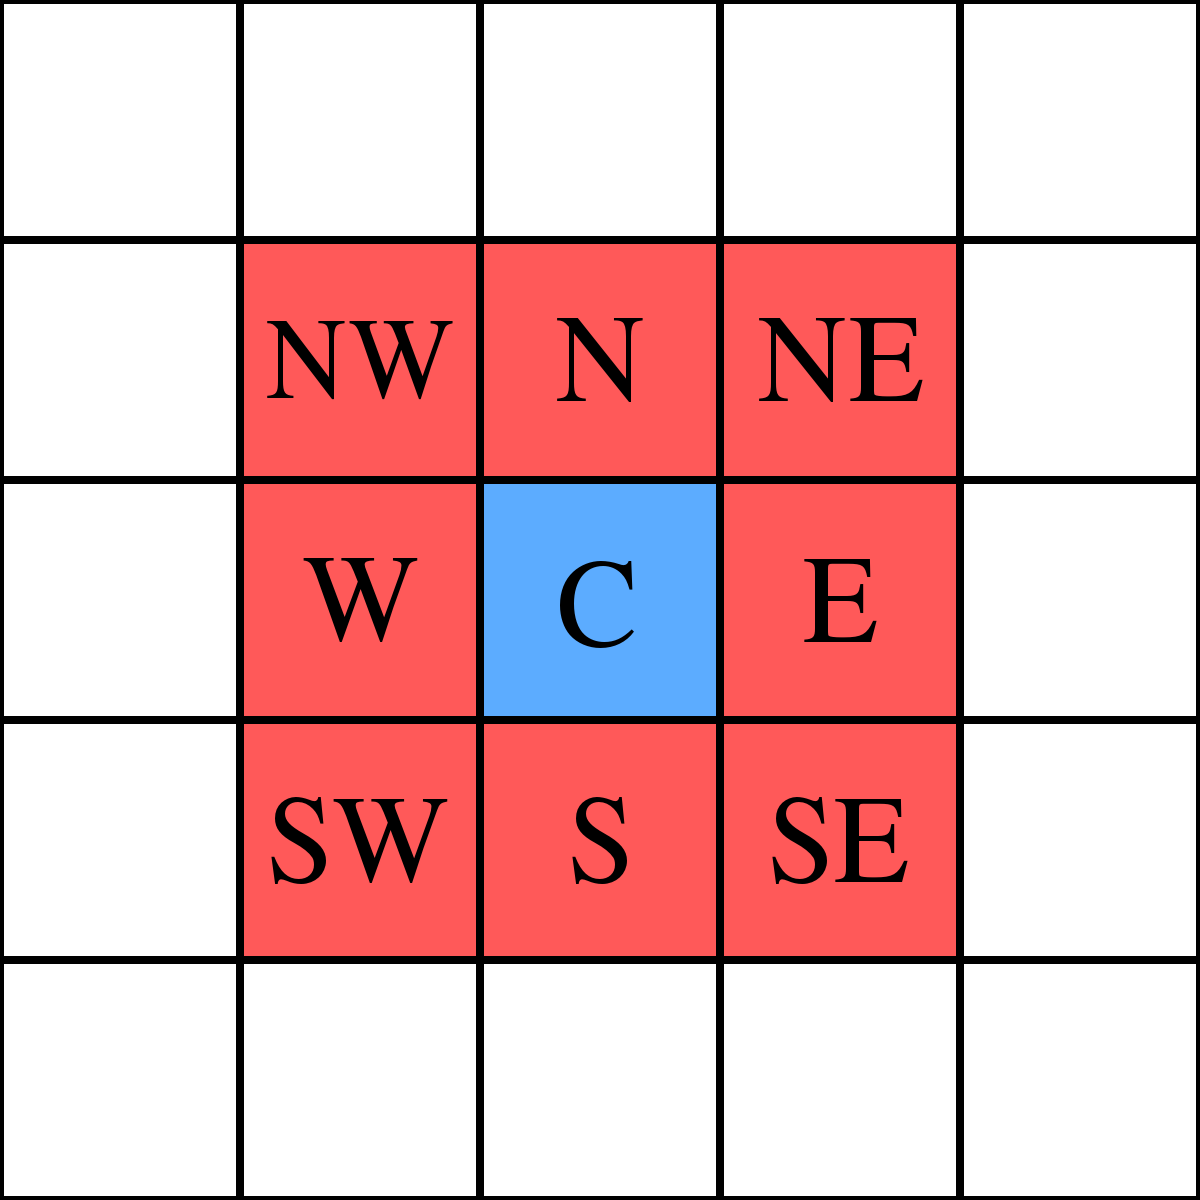
\includegraphics[scale=0.075]{moore_n.png}
\end{figure}
\\
Moore-type neighbourhoods can additionally consider a specific range or depth.
\begin{figure}[h]
    \caption{Moore Neighbourhood with Ranges \cite{wolfram}}
    \centering
    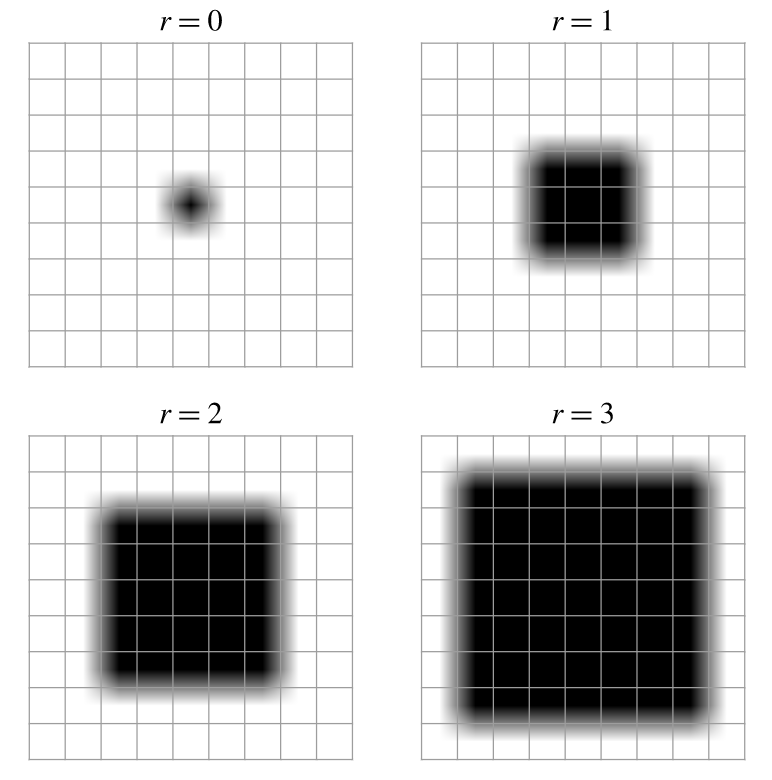
\includegraphics[scale=0.70]{moore_n_ranges.png}
\end{figure}
\\
\newpage
\section{Existing Applications of 2D Cellular Automata}
CAs have been implemented in a vast number of fields due to its reliance on relatively simple rules. These fields are briefly touched upon in the first chapter of this report. Furthermore, applying cellular automata on different areas of knowledge rely on manipulating the rules. This would suggest quite a substantial devation in rules when compared to conventional, more popular CAs such as Conway's Game of Life.

\subsection{Conway's Game of Life}
Conway's Game of Life (henceforth CGOL) is a two-state CA with a special set of transition rules. Developed by John Conway in 1970, CGOL is arguably the most popular two-dimensional cellular automaton \cite{gardner10fantastic}. It is an example of an outer totalistic CA. State transitions rely on Moore-type neighbourhoods, with deterministic rules. 
\\ \\
The state transition rules for each cell in a CGOL can be written in the form of if-statements:

\begin{itemize}
    \item \textbf{IF} the cell is \textit{alive} and has two or three live neighbours, \textbf{THEN} it remains alive in the next generation
    \item \textbf{IF} the cell is \textit{dead} and has exactly three live neighbours, \textbf{THEN} it becomes a live cell in the next generation
    \item \textbf{ELSE} the cell dies, or stays dead
\end{itemize}
Otherwise the following flowchart visualizes how the rules may work:
\begin{figure}[H]
    \caption{CGOL Rules Flowchart}
    \centering
    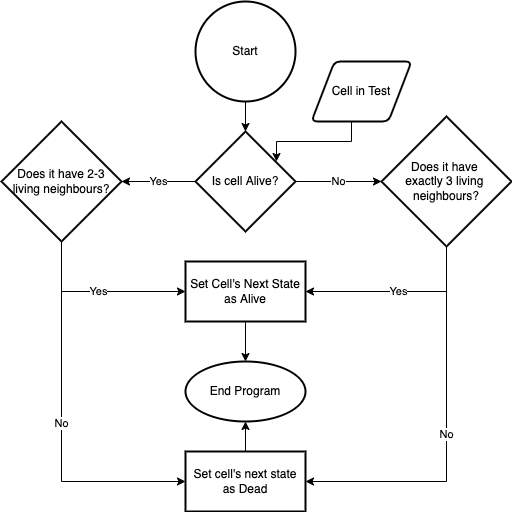
\includegraphics[scale=0.50]{flowchart_cgol.drawio.png}
\end{figure}
\noindent CGOL is Turing Complete. \cite{rendell2010simple}. The universality proof of CGOL in being Turing Complete was demonstrated by creating signals using the aforementioned Gliders, and combining them to create conventional logic gates (i.e. AND, OR, NOT) \cite{rendell2002turing}. 

\subsection{Forest Fire Propagation}
CAs have extensively been applied in forest fire propagation. Their models typically implement two-dimensional probabilistic cellular automata with three or more states. The CA model outlined by \cite{alexandridis_2011} make use of a square grid, with a potential of fire propagating to its eight nearest neighbours (i.e. Moore-type neighbourhoods). The rules according to the aforementioned journal are as follows:
\begin{enumerate}
    \item A cell that cannot be burnt stays the same
    \item A cell that is currently burning down will completely burn down at the next state
    \item A burned cell cannot burn again
    \item If a cell is currently burning, and its neighbours include cells containing vegetative fuel (i.e. 'burnable' state), then the fire can propagate to said neighbour with a certain probability. 
\end{enumerate}
The probability in this case may be affected by a myriad of factors. The article by Freire \cite{freire} has modelled propagation probabilities based on wind, slope shape, and vegetation density. 
\\ \\
The CA model outlined above, with probability functions integrated in its transition rules, is used to simulate the 2012 Algarve fire of Southern Portugal \cite{freire}. The same model, after a number of simulations, has also demonstrated an added value to assist in firefighting resource allocation in the event of a forest fire \cite{freire}.

\subsection{Population Dynamics}
In the study by Mavroudi \cite{mavroudi}, CAs were used to model population dynamics in the city of Salonica, Greece. Most CAs that are purposed to modelling population growth are mostly developed through trial and error (essentially heuristics) \cite{wu2002calibration}. In the context of city development, the rules in this CA are heavily influenced by its ecosystem. No city is regular, and these organic growths in population are usually affected by historical events and random decision making. \cite{batty1997cellular}. CAs have been used in urban population predictions since the late 1980s \cite{batty1999modeling}. 
\\ \\
Regarding urban growth and development, the CA rules are still a research topic \cite{batty1998urban}

\subsection{Game Development: 2D Map Generation} \label{gamedevimp}
Two-dimensional maps in games can often generated using CA. One of the CAs that can be used for map generationcan be a two-dimensional, two-state totalistic CA with deterministic state transition rules observing their Moore Neighbourhoods \cite{johnson2010cellular}. A common rule according to Johnson \cite{johnson2010cellular} for two-dimensional map generation is as such: 
\begin{itemize}
    \item \textbf{IF} a cell has more than four \texttt{wall} neighbours, \textbf{THEN} it turns to a \texttt{wall}
    \item \textbf{ELSE} the cell turns to a \texttt{floor}
\end{itemize}
\noindent The above is commonly used as cavern system generations in a game \cite{ashlock2015evolvable}. Another implementation of CAs in Game Development is a three-state genotype-to-phenotype based CA to recreate the Dune 2 Real-Time-Strategy map. In this implementation, however, the map is generated via genotype represented by matrices. CAs are only used here to create higher resolution maps through a stochastic process \cite{mahlmann2012spicing}. 

\section{Potentially Useful External Libraries and Tools}
To streamline the project development process, there are a number of libraries that may help as building blocks for the end product:

\subsection{JSON and JSON Schema} \label{json_schema}
JSON (short for JavaScript Object Notation) is a common data interchange format. JSON can contain JSON entities on its own, and is easy for humans to write, and computers to parse \cite{bassett2015introduction}.
\\ \\
JSON Schema on the other hand is a special type of JSON that can be used to validate whether another JSON meets the requirements specified on the schema. It is a schema language. Validators typically validate JSON entities against a schema that is supplied, such as in a MongoDB database instance or API requests \cite{pezoa2016foundations}.
\\ \\
Essentially, JSON Schema is a response to the lack of standardized metadata or schema language for JSON - the most popular data format for API requests and responses. However, this is still under research and development \cite{pezoa2016foundations}. 

\subsection{P5JS} \label{p5js}
P5JS is a JavaScript library, utilized for ’creative coding’. This library is targeted primarily for audiences with an intent to draw, and therefore a myriad of its keywords rotate on the concept of sketching and drawing on a canvas \cite{mccarthy2015p5js}. This library may be useful in visualizing the CA.

\subsection{TV4} \label{tv4}
Tiny Validator 4 (TV4) is a JS library written for use with JS or HTML/JS applications (typical installation using NPM or Yarn) \cite{tv4}. This library enables the use of JSON validation with a specified JSON Schema. If there were a validator component in the project, this library will surely prove useful. 

\subsection{Git, GitHub and GitHub pages}
Every step of the development process is synchronized with GitHub version control. Proper workflow is maintained to the best of my abilities, and this has made the development process easier. The final project is hosted on GitHub pages for everyone to see and to provide room for evaluation, using a custom subdomain purchased from Namecheap. The project can be found at \texttt{https://projects.rakhadjo.me/y3-project}